\documentclass{article}
\usepackage[utf8]{inputenc}
\usepackage[L7x]{fontenc}
\usepackage[lithuanian]{babel}
\usepackage{lmodern}
\usepackage{amsmath}
\usepackage{graphicx}
\usepackage{verbatim}
\usepackage{hyperref}
\usepackage{tcolorbox}
\usepackage{mdframed}
\usepackage{tikz}
\usepackage{cancel}
\usepackage{color}
\usepackage[top=2cm, bottom=2cm, left=2cm, right=2cm, footskip=1cm, a4paper]{geometry}
\usepackage{hyperref}
\usepackage[upint]{stix}
\usepackage{amsthm}
\usepackage{indentfirst}
\usepackage{enumitem}
\usepackage{framed}
\usepackage{tasks}

\begin{document}
\tableofcontents{}
\section*{Klausimai mokytojams. Apie matematikos istoriją}

\textbf{Iki renesanso} - kaip atrodė matematika ir joje iškilę sunkumai, skaitykite \href{http://norvaisa.lt/matematika/mokykline-matematika/kodel-neigiamuju-skaiciu-sandauga-yra-teigiamas-skaicius/}{čia}. 

\textbf{Naujų žymėjimų atsiradimas} - skaitome \href{http://jeff560.tripod.com/operation.html}{čia} ir \href{https://www.math.ucdavis.edu/~anne/WQ2007/mat67-Common_Math_Symbols.pdf}{čia}.

Algebriniai pertvarkymai, kuriuos dabar mokosi moksleiviai, sukurti daugiausia renesanso laikotarpiu. Čia apžvelgiu svarbiausius įvykius, kurie galėtų būti įtraukti į klausimus mokytojams

\textbf{1489m.} + ir - ženklai pirmąsyk pasirodo matematiniuose darbuose. Jie reiškia perviršį ir likutį.

\textbf{1515m.} del Ferro randa kubinės lygties sprendinį, tačiau jo sprendimas lieka niekam nežinomas.

\textbf{1525m.} Pirmąsyk panaudojamas simbolis $\sqrt{}$, reiškiantis kvadratinę šaknį.

\textbf{1535m.} Tartaglia taip pat randa kubinės lygties $x^3=ax+b$ sprendinį ir jį, paprašytas Kardano, atskleidžia su prašymu neviešinti informacijos, kol jis pats jos nepublikuos.

\textbf{1545m.} Pasirodo Kardano rašyta knyga \textit{Ars Magma}, turėjusi didelę istorinę svarbą ankstyvajame renesanse. Joje Kardanas paskelbia savo darbą su kitų tipų kubinėmis lygtimis (pvz. $x^3+ax^2=b$ ir pan.) pratęsdamas Tartaglios metodus. Sprendimą paskelbti Tartaglios metodus jis motyvavo tuo, kad jo taikytos formulės buvo jau žinomos del Ferro. Knygoje taip pat įtrauktas Kardano studento Ferrari sprendimas ketvirto laipsnio lygtims, kuriam būtina naudoti Tartaglia metodą. Visose lygtyse pagal ano meto matematiką leistina naudoti tik teigiamus koeficientus, nes neigiami skaičiai laikyti apgaulingais, tačiau Kardanas - pirmasis Europos matematikas, pasiūlęs, kad tie patys skaičiavimai gali būti atlikti su koeficientais nepriklausomai nuo jų ženklo. Taip pat jis pirmąsyk istorijoje panaudojo kompleksinius skaičius: vienoje knygos dalyje yra parodyta, kaip atlikti veiksmą $(5+\sqrt{-15})(5-\sqrt{-15})$. Kaip tuo metu būdavo užrašomi reiškiniai, galite pamatyti \href{http://www.ms.uky.edu/~sohum/ma330/files/eqns_2.pdf}{šičia, 4psl}. Sklaustai ligi 18 amžiaus matematikoje - retenybė.

\textbf{$\approx$ 1557-60m.} Matematiniuose darbuose pasirodo =, >,< ženklai vietoj frazių ,,lygu su'', ,,daugiau už'' ir ,,mažiau už'' vartojimo.

\textbf{1591m.} Vijetas parodo, kad kubinės lygties išsprendimo uždavinys yra ekvivalentus su antikiniu kampo dalijimo į 3 dalis uždaviniu. 

\textbf{1628m.} Matematiniuose darbuose pirmąsyk pasiūlomas modulio ženklas.

\textbf{1629m.} ir \textbf{1637m.} Nepriklausomuose Ferma ir Dekarto darbuose pirmąsyk aptariamas geometrinių kreivių naudojimas koordinačių sistemoje (algebra naudojama spręsti geometriniams uždaviniams ir atvirkščiai). Pavyzdžiui kubo padvigubinimo uždavinys ($x^3=2$) sprendžiamas sukertant parabolę $y=\frac{x^2}{2}$ ir hiperbolę $y=\frac{1}{x}$, o ketvirto laipsnio lygtis $x^4=ax^2+bx+c$ sprendžiama sukertant parabolę $y=x^2$ su parabole $x=\frac{y^2-ay-c}{b}$. Dar pusantro amžiaus lygčių sprendimas buvo paliktas algebrai, konstravimo uždaviniai - Euklido geometrijai, o algebrinė geometrija buvo teorija apie kreives.

\textbf{1629m.} Pasiūlyta naudoti šaknį su indeksu.

\textbf{1631m.} Matematiniuose darbuose pasirodo $\pm$ ženklas,

\textbf{1633m.} Matematiniuose darbuose pasirodo ,,:'' ženklas, naudojamas trupmenoms aprašyti.

\textbf{1634-37m.} Matematiniuose darbuose pasirodo dabartinis laipsnio žymėjimas.

\textbf{1637m.} Dekartas pasiūlo naudoti pilną šaknies žymėjimą ($\sqrt{\phantom x}$)

\textbf{1640m.} Ferma įrodo Mažąją Ferma Teoremą panaudodamas binominius koeficientus. Jis yra vienintelis renesanso laikų  mokslininkas, tyrinėjęs skaičių teoriją, tačiau daugelis jo prieitų rezultatų buvo gauti neaprašant naudojamų metodų. Jo išvadų ir hipotezių įrodymai buvo palikti Oileriui, Lagrandžui ir Ležanrui. 

\textbf{1654m.} Paskalis, nagrinėdamas binominių koeficientų savybes, savo darbuose pirmąsyk panaudoja dabartinę indukcijos (pradinis žingsnis - indukcinis žingsnis) konstrukciją, tačiau dar pora šimtų metų niekas nesuformuluoja sprendimuose naudojamo indukcinio samprotavimo sąvokos.

\textbf{1658m.} Matematiniuose darbuose pasirodo ,,÷'' ženklas, naudojamas dalinimo operacijai aprašyti.

\textbf{1684m.} Leibnicas panaudoja ,,:'' ženklą, reiškiantį ir trupmeną, ir dalinimo operaciją.

\textbf{1698m.} Savo laiške Paskaliui Leibnicas pasiūlo naudoti $\cdot$ ženklą.

\textbf{1733 m.} Į Lietuvą pakliūna pirmasis algebros vadovėlis \textit{Alpha matheseos}.

\textbf{1755m.} Oileris panaudoja sumavimo simbolį $\sum$.

\textbf{1761m.} Oileris panaudoja atvirštinio daugiklio sąvoką Mažosios Ferma Teoremos įrodyme.

\textbf{1796m.} Gausas sukonstruoja 17-kampį vien su apskritimais ir tiesėmis - figūrą, nenagrinėtą Senovės Graikų. Tai nulemia jo apsisprendimą tapti matematiku. Jis susidomi Oilerio, Lagrandžo ir Ležanro darbais ir jų neišspręstais uždaviniais. Dar po 5 metų jis išleidžia knygą \textit{Disquisitiones Arithmeticae}, kurioje vysto teoriją apie visus taisyklinguosius $n$-kampius. Ši knyga svarbi tuo, kad prisidėjo prie rimtesnių skaičių teorijos pokyčių ir moderniosios algebros atsiradimo, į kurią įeina abstrakčios daugianarių savybės. Į knygą taip pat įeina:
\begin{itemize}
\item įrodymas, kad kiekvieną skaičių galima išskaidyti pirminiais dauginamaisiais vieninteliu būdu;
\item apibrėžiama lyginio sąvoka ir pasiūloma ją panaudoti įsitiknant, kad visos daugianario $x^3-8x+6$ liekanos yra nenulinės dalijant iš 5.
\end{itemize}

\textbf{1837m.} Nežymus matematikas Wantzel pirmasis įrodo, kad kubo padvigubinimo ir kampo dalijimo į tris lygias dalis uždaviniai yra neišsprendžiami geometriniais konstravimais, papildo Gauso taisyklingųjų $n$-kampių teoriją ir patikslina (Dekarto darbe 1637m. tik numanomus) algebrinius sukonstruojamumo kriterijus.

\textbf{1838-39m.?} Dirichle apibrėžia algebrinio skaičiaus sąvoką ir ją naudoja plėtojant algebrinę skaičių teoriją.

\textbf{1857m.} Dedekindas pasiūlo vietoje lyginių (kongruentumo sąryšių) naudoti kongruentumo klases kaip algebrinius objektus.

\textbf{1858m.} Dedekindas pasiūlo iracionaliuosius skaičius aiškinti ne remiantis atkarpomis pagal Eudoxo (350m. p.m.) plėtotą proporcijų teoriją, o naudojant racionaliųjų skaičių aibes.

\textbf{1872m.} galiausiai Dedekindas pasiūlo realiųjų skaičių aibę tapatinti su skaičių tiese. Tai nepaprastos svarbos prielaida, nes geometrinę tiesę ir realiųjų skaičių aibė gali būti laikytini abipus vienareikšmėje atitiktyje. Savo prielaidoje Dedekindas naudoja tokius apibrėžimus: 
\begin{itemize}
\item iracionalusis skaičius $\lambda$ - tai racionaliųjų skaičių aibės $\mathbb{Q}$ padalijimas į du poaibius $L_\lambda$ ir $R_\lambda$, tokius, kad kiekvienas $L_\lambda$ narys yra mažesnis už $R_\lambda$ narį, poaibis $L_\lambda$ neturi didžiausio nario, o poaibis $R_\lambda$ neturi mažiausio nario. Negriežtai į skaičių $\lambda$ galime žiūrėti kaip į skylę tarp šių poaibių. 
\item Šiame apibrėžime išėmę sąlygą ,,$R_\lambda$ neturi mažiausio nario'' gauname realiųjų skaičių apibrėžimą.
\end{itemize}
Tolimesni uždaviniai suformulavus šią prielaidą yra apibrėžti realiųjų skaičių sąryšius ir operacijas naudojant aibes. Pavyzdžiui:
\begin{itemize}
\item Jei $a < b$, tai $L_a\subseteq L_b$ ir $L_a\neq L_b$
\item Jei $a\le b$, tai $L_a\subseteq L_b$
\end{itemize}

\textbf{1882m.} Lindermannas išsprendžia paskutiniąją iš trijų antikinių problemų - kvadrato, lygiapločio su skrituliu sukonstravimo klausimą. Jis parodo, kad skaičius $\pi$ ne tik negali būti gaunamas geometriniu konstravimo būdu, bet netgi negali būti kurio nors daugianario reikšmė, su kuria jis lygus 0, t.y. išreikštas radikalais.

\textbf{1888m.} Dedekindas apibrėžia uždarinio sąvoką ir ją panaudodamas apibrėžia natūraliuosius skaičius kaip aibės $\{0\}$ uždarinį virš operacijos ,,+1''. Ši natūraliųjų skaičių samprata yra būtina dabartiniam indukcijos modeliui apibrėžti. Ji lemia esminius pokyčius skaičių teorijoje, nes natūraliųjų skaičių operacijas + ir $\times$ jau galima apibrėžti induktyviai, be to, skaičių teorija tampa neatsiejama nuo aibių teorijos. 

\textbf{1890m.} Pirmąsyk panaudojamas $\subset$ simbolis.

\textbf{1917m.} Pirmąsyk mokyklose pasiūloma naudoti skliaustus, kad būtų išvengta nesusipratimų su operacijų eiliškumu.

\textbf{1921m.} Išleistas pirmasis algebros vadovėlis lietuvių kalba.

\section*{Klausimai mokytojams ir mokiniams. Apie matematines sąvokas}
Čia pateiksime pavyzdžius uždavinių, kuriais būtų ugdomas ne gebėjimas atlikti mokyklines procedūras, o gebėjimas naudotis matematinėmis sąvokomis.
\begin{enumerate}
\item Senovės Graikijoje buvo vartojama tokia Pitagoro teoremos formuluotė: \texttt{Kvadratas ant stačiojo trikampio įžambinės BC yra suma kvadratų ant trikampio statinių BA ir AC}. Pabandykite tą pačią mintį išreikšti taisyklingiau vartodami šiuolaikinę matematinę kalbą.
\item \textit{Elementai} - tai didžiausią įtaką matematikos vystymuisi padaręs vadovėlis, išleistas maždaug 300m. prieš mūsų erą senovės graikų matematiko Euklido. Jame pateikti tokie sąvokų apibrėžimai:
\begin{itemize}
\item \textit{Vienetas yra tai, kas pagal prigimtį egzistuoja kaip vienas daiktas.}
\item \textit{Skaičius yra vienetų daugis.}
\end{itemize}
Palygink, kuo ši skaičiaus samprata skiriasi nuo dabartinės skaičiaus sampratos. Gali remtis angliškoje Vikipedijoje nurodytu skaičiaus apibrėžimu:
\begin{itemize}
\item Skaičius yra matematinis objektas, naudojamas skaičiavime, matavime arba numeravime.
\end{itemize}
\item Įvardykite matmenis šių geometrinių objektų: \texttt{atkarpa, kubas, kvadratas, kampas}.
\item Matmenys, kuriuos įvardijote ankstesniame pratime, antikinėje matematinėje kalboje nebuvo vartojami. Remdamiesi šiuo teiginiu paaiškinkite, kodėl Senovės Graikijos matematikai nenustebtų išgirdę pirmame uždavinyje paminėtą formuluotę.
\item Duotas matematinių objektų rinkinys: \texttt{skaičius}, \texttt{taškas}, \texttt{tiesė}, \texttt{aibė}
Suskirstykite juos į dvi grupes pagal panašumą ir tą panašumą apibūdinkite.
\item Ar egzistuoja
\begin{enumerate}
\item  taškas, kuris nepriklauso tiesei?
\item  taškas, kuris nepriklauso jokiai tiesei?
\item aibė, sudaryta ne iš skaičių?
\item  skaičius, kuris nepriklauso realiųjų skaičių aibei?
\item  atkarpa, kuri nepriklauso kitai atkarpai?
\item  atkarpa, kuri nepriklauso jokiai kitai atkarpai?
\item  aibė, kuri priklauso kitai aibei?
\item  aibė, kuri nepriklauso jokiai kitai aibei?
\item  tiesė, kertanti kitą tiesę daugiau nei viename taške?
\end{enumerate}
\item Duoti skaičiai -0,32 ir -0,18. Užrašykite šių skaičių sumos ir skirtumo sandaugą ir apskaičiuokite sudaryto reiškinio reikšmę.

\item Įrodykite, kad bet kuriems dviems skaičiams $a$ ir $b$ visada galioja teiginys: \texttt{jų sumos kvadrato ir jų skirtumo kvadrato suma yra nemažesnė už jų kvadratų sumos ir bet kurio iš jų kvadrato sumą.}

\item Kiek skaičiaus 2018 užraše yra skaitmenų porų, tokių, kad poros narys, skaičiaus užraše esantis pirmiau likusio poros nario, yra už tą narį didesnis?

\item Kada dviejų skaičių kvadratų santykis nėra lygus jų santykio kvadratui?

\item Koks raidinis reiškinys atitinka sakinį \texttt{skaičių a ir b sumos kvadrato ir šių skaičių kvadratų sumos dalmuo?}

\item  Lentoje ant kvadrato viršūnių yra surašyti tam tikri skaičiai, lygūs $a$, $b$, $c$ ir $d$. Bonifacijus atsitiktinai pasirinko vieną iš sudėties ir daugybos operacijų, o paskui ją atlikęs su kiekviena iš gretimose viršūnėse esančių skaičių porų, lentoje užrašė 4 tos operacijos rezultatus. Tada vėl pasirinko vieną iš sudėties ir daugybos operacijų ir ją atlikęs su šiais 4 rezultatais gavo tam tikrą skaičių. 
\begin{tasks}(1)
\task Užrašykite reiškinius, atitinkančius visas galimas šio skaičiaus išraiškas.
\task Nustatykite visas galimas skaičių $a$, $b$, $c$ ir $d$ sumos reikšmes, jei gautasis skaičius lygus 2018.
\end{tasks}

\item Pateikite būdą, kaip bet kuriam racionaliajam skaičiui sudaryti lygtį, kuriai šis skaičius yra sprendinys.

\item Kaip vadinama aibė skaičių, gautų kiek nori kartų naudojant 1 ir leistinas operacijas, jei:
\begin{tasks}(2)
\task leidžiama tik operacija +; 
\task leidžiamos tik operacijos + ir -; 
\task leidžiamos tik operacijos +, - ir $\times$; 
\task leidžiamos tik operacijos +, -, $\times$ ir : ? 
\end{tasks}
\item Įrodykite, kad tarp bet kurių dviejų skirtingų realiųjų skaičių egzistuoja
\begin{tasks}(2)
\task racionalusis skaičius.
\task iracionalusis skaičiius
\end{tasks}
\end{enumerate}

\section{Du matematinių sąvokų įsisavinimo būdai}

\textit{\textbf{Kategorizavimas}} yra pirmasis būdas suprasti matematinėms sąvokoms, įgyjamas per matematinių objektus ir jų savybių tyrinėjimą ir besivystantis kartu su vis tikslesnės kalbos vartojimu. Šiuo atveju matematinė sąvokos supratimą galime laikyti pilnu, kuomet:
\begin{itemize}
\item gebama ją apibrėžti naudojantis kitomis matematinės sąvokomis. 
\item apibūdinami objektai priklauso tai ir tik tai kategorijai objektų, kurie įeina į apibrėžimą. 
\end{itemize}

\textbf{\textit{Enkapsuliacija}} yra antrasis būdas suprasti matematinėms sąvokoms, įgyjamas atliekant matematines procedūras tol, kol atlikimas tampa savaiminiu, pastangų nereikalaujančiu procesu, o pats procesas imamas suprasti kaip naujas objektas. Šiuo atveju matematinė sąvokos supratimą galime laikyti pilnu, kuomet:
\begin{itemize}
\item gebama suprasti žingsnius, kurie yra būtini nagrinėjamai procedūrai atlikti.
\item reiškinys suprantamas ne tik kaip procedūra (pažingsninė instrukcija rezultatui gauti), tačiau ir kaip matematinis objektas, kurio rezultatas nėra aktualus tam, kad jį galėtume naudoti kitų sąvokų ar procedūrų kontekste. Pavyzdžiui šaknis, trupmena arba suma.
\end{itemize}

Čia pateiksiu pavyzdį, parodantį, jog šaknies sąvokos supratimas yra vienas iš unikalių pavyzdžių, kuomet reikia panaudoti ir kategorizaciją, ir enkapsuliaciją.

Šaknį iš skaičiaus $a$ \textbf{\textit{apibrėžiame}} kaip skaičių, kurį sudauginę su savimi, gausime skaičių $a$. Šis apibrėžimas būtų neteisingas, nes pagal jį šaknis iš 9 galėtų būti ne tik 3, o -3. Tai pastebėję, apibrėžimą patiksliname: nurodome, kad skaičius, dauginamas su savimi, privalo būti teigiamas. Toks šaknies supratimas yra įgyjamas \textit{\textbf{kategorizavimo}} būdu. 

Vis dėlto moksleiviai dažnai pasimeta, kai reikia ištraukti šaknį iš 2. Remiantis šaknies apibrėžimu, reikia sugalvoti skaičių, kurį padauginę iš savęs gausime 2. Mokykliniame turinyje nėra jokios procedūros, kurios laikantis tokį skaičių būtų galima rasti. Reiktų pamėginti bent vieną procedūrą. Aš siūlau \textbf{\textit{spėjimo - tikrinimo}} metodą:

\begin{itemize}
\item $1\times 1=1$ - tai, ką spėjome, buvo per mažas skaičius
\item $2\times 2=4$ - 2 - tai, ką spėjome, buvo per didelis skaičius. Imame vidurį tarp 1 ir 2.
\item $1,5\times 1,5=2,25$ - tai, ką spėjome, buvo per didelis skaičius. Imame vidurį tarp 1 ir 1,5.
\item $1,3\times 1,3=1,69$ - tai, ką spėjome, buvo per didelis skaičius. Imame vidurį tarp 1,3 ir 1,5.
\item $1,4\times 1,4=1,96$ - tai, ką spėjome, buvo tik beveik. Reikia šiek tiek didesnio skaičiaus.
\item $1,41\times 1,41=1,9881$ - spėjimas dar vis per mažas. Reikia šiek tiek didesnio skaičiaus.
\item $1,42\times 1,42=2,0164$ - spėjimas jau per didelis. Imame vidurį tarp 1,41 ir 1,42.
\item $1,415\times 1,415\dots$
\end{itemize}
 
Iš tiesų ši procedūra yra begalinė, todėl tikslaus rezultato niekad negausime. Kalkuliatorius rodo, kad $\sqrt{2}=1,414213562373095$, tačiau skaitmenų yra be galo daug ir teisinga būtų rašyti $\sqrt{2}=1,414213562373095\dots$
 
Pateikta situacija, kuomet tikslus rezultatas neegzistuoja, atspindi, kodėl $\sqrt{2}$ prasminga suprasti kaip savitą objektą, o ne kaip procedūrą. Priešingai nei atveju $\sqrt{9}$, kuomet rezultatas egzistuoja. \textit{\textbf{Kategorizavimo}} būdu, į kurį įeina gebėjimas pasiremti šaknies apibrėžimu, galima suprasti, kad objektas $\sqrt{2}$ tenkina lygybę $\sqrt{2}\times \sqrt{2}=2$. \textbf{\textit{Enkapsuliacijos}} būdu suprantame, kad tai yra objektas, o ne procedūra.

Panašias išvadas galime gauti ir skaičiaus $\frac{1}{7}$ atveju. Kai kurios trupmenos, tokios kaip $\frac{3}{4}$, gali būti laikomos turinčiomis rezultatą (šiuo atveju 0,75). Procedūra, kurią panaudojame rezultatui gauti, šįsyk galėtų būti ne \textbf{\textit{spėjimo - tikrinimo}} metodas, o \textbf{\textit{dalyba kampu.}} Tačiau skaičiaus $\frac{1}{7}$ atveju, kaip ir $\sqrt{2}$ atveju, reikia panaudoti ir kategorizaciją, ir enkapsuliaciją. 
 
Šie pavyzdžiai parodo, kodėl nemaža dalis moksleivių objektų $\frac{1}{7}$ ir $\sqrt{2}$ nelaiko skaičiais, o skaičiais laiko tik dešimtaines trupmenas, tokias kaip 12,904. Jei skaičius būtų apibrėžiamas kaip dalykas, kuriam apskaičiuoti egzistuoja baigtinė procedūra, tuomet moksleiviai būtų teisūs. Tačiau skaičius kartu yra ir \textit{\textbf{abstrakcija}} - mintinis objektas, kurio sąvoka ir savybės yra išvestos iš tam tikrų skaičiavimo pavyzdžių, tačiau mąstant apie šį objektą skaičiavimai neatliekami.

\section{Kategorizacija}
\subsection{Bandymas įvartinti ir klasifikuoti matematines sąvokas pagal griežtumą}
Neišvengiamą susidūrimą su prieš tai neapibrėžtomis sąvokomis apibūdina \textit{Gilbert de B. Robinson}:

\textit{Ne matematikams dažnai atrodo keista, jog neįmanoma aiškiai apibrėžti visų matematikoje vartojamų terminų. Ši problema nėra paviršutinė. Ji glūdi pažinimo gelmėse. Norint pažinti būtina nuo kažko pradėti ir norint, jog pažinimas vystytųsi, būtina aiškiai nurodyti, kurie objektai ir jų sąryšiai negali būti apibrėžti. Tuomet jų savybes mes priimsime kaip suprantamas intuityviai.}
\begin{mdframed}[backgroundcolor=blue!10!white, linewidth=3pt]
Sąvoką laikome \textit{\textbf{primityvia}}, jei jos negalima apibrėžti remiantis prieš tai apibrėžtomis matematinėmis sąvokomis. Sąvoką laikome \textit{\textbf{matematiškai apibrėžiama}}, jei ją galima apibrėžti remiantis prieš tai apibrėžtomis matematinėmis sąvokomis. 
\end{mdframed}
Pateiksime pavyzdį kaip apibrėžiant sąvoką \textit{\textbf{kraštinė}} galime pamatyti, kokios kitos sąvokos yra būtinos joms apibrėžti ir kaip jas galima suskirstyti į \textit{\textbf{apibrėžiamas}} ir \textit{\textbf{primityvias}}.

\colorbox{green}{Kraštinė} - tai \colorbox{green}{atkarpa}, \colorbox{yellow}{apribojanti} \colorbox{cyan}{plokštumos} \colorbox{orange}{figūrą}.

\colorbox{green}{Atkarpa} - tai \colorbox{cyan}{tiesės} \fbox{dalis}, \colorbox{yellow}{apribota} \fbox{dviejų} \colorbox{cyan}{taškų} ir \colorbox{cyan}{esanti tarp} jų.

\colorbox{orange}{Figūra} - tai \colorbox{cyan}{geometrinis objektas}, \fbox{turintis} \colorbox{orange}{formą}.

\colorbox{orange}{Objektas} - tai, į ką nukreipta pažintinė veikla.

\colorbox{orange}{Geometrija} - tai matematikos šaka, tyrinėjanti figūras bei jų padėtį, dydžius ir erdvės savybes.
\newline

Čia naudojamas spalvinimas atspindi keturias pagrindines matematinių sąvokų rūšis:
\begin{itemize}
\item \colorbox{green}{Žalia spalva} žymimos matematiškai apibrėžiamos sąvokos.
\item \colorbox{cyan}{Mėlyna spalva} žymimos primityvios sąvokos.
\item \colorbox{orange}{Oranžine spalva} žymimos buitinės sąvokos, kurių matematiškai apibrėžti negalime.
\item \colorbox{yellow}{Geltona spalva} žymimos sąvokos, kurias moksleiviai pagal mokyklinę programą gali suvokti tik buitiškai, nors joms egzistuoja matematiniai apibrėžimai, besiremiantys nemokyklinės matematikos teorija. 
\item \fbox{Apibraukti} žodžiai sąvokomis nelaikomi. Jie atitinka \textbf{\textit{kvantorius}}.
\end{itemize}

Matematiškai apibrėžiamai sąvokai būdinga tai, kad vienareikšmiškai galima pasakyti ar apibrėžiamas objektas atitinka sąvoką. To negalėtume pasakyti apie buitines sąvokas, kurias kasdieniniame gyvenime nėra įprasta vienareikšmiškai apibūdinti. Pavyzdžiui, pilies sąvoka enciklopedijoje apibūdinama taip: uždaras gynybinių įrenginių bei gyvenamujų, ūkinio, kulto ir kt. pastatų kompleksas. Gedimino pilis yra objektas atitinkantis pilies sąvoką. Tačiau apie daugelį objektų Vilniuje ir jo apylinkėse būtų sunku vienareikšmiškai tvirtinti, ar tai yra pilis, ar ne. Tuo labiau pilių rinkinys: \textit{visos Vilniaus rajono pilys, turinčios raudoną stogą} nėra vienareikšmiškai apibrėžtas. 

Savybę, jog matematiškai apibrėžta sąvoka išlaiko vienareikšmiškumą, galima taikyti tiriant, ar įvairūs apibrėžimai pilnai atitinka tiriamą sąvoką. 

\textbf{\textit{1 Pavyzdys.}} Šaknis iš skaičiaus $a$ - tai toks skaičius $b$, kurio kvadratas lygus $a$.

Imkime $a=9$ ir $b=-3$. Šie skaičiai atitinka aibrėžimo sąlygas, tačiau -3 nėra šaknis iš 9. Vadinasi, šaknies apibrėžimą reiktų pakeisti (galima nurodyti, jog $b$ teigiamas).

\textbf{\textit{2 Pavyzdys.}} Atkarpa - tai tiesės dalis, esanti tarp dviejų taškų.

Imkime tiesę, kuri yra skaičių ašis, intervalų sąjungą $(1;2)\bigcup (3;4)$ bei du taškus, atitinkančius skaičių ašyje skaičius 0 ir 5. Akivaizdu, kad ši intervalų sąjunga nėra atkarpa, tačiau atitinka apibrėžimo sąlygas. Vadinasi, atkarpos apibrėžimas buvo netikslus: jis \textbf{\textit{apima}} ir geometrinius objektus, sudarytus iš ,,skylėtų'' tiesės dalių.

\textbf{\textit{3 Pavyzdys.}} Atkarpa - tai tiesės dalis, apribota dviejų taškų.

Imkime tiesę, kuri yra skaičių ašis, intervalų sąjungą $(-\infty;2)\bigcup (3;+\infty)$ bei du taškus, atitinkančius skaičių ašyje skaičius 2 ir 3. \colorbox{yellow}{Apriboja} yra ,,geltonasis'' žodis, t.y. moksleiviai jį gali suprasti tik buitiškai. Pagal buitiškai suvokiamą prasmę būtų galima taip samprotauti: spindulys turi vieną apribojantį tašką, atkarpa - du, intervalų sąjunga $(-\infty;2)\bigcup (3;+\infty)$ skaičių ašyje - keturis. Akivaizdu, kad ši intervalų sąjunga nėra atkarpa, tačiau atitinka apibrėžimo sąlygas. Vadinasi, atkarpos apibrėžimas buvo netikslus: jis apima ir geometrinius objektus, esančius už ,,ruožo'' tarp dviejų taškų.

\textbf{\textit{4 Pavyzdys.}} Atkarpa - tai tiesės dalis, apribota dviejų taškų ir esanti tarp jų. 

Imkime tiesę, kuri yra skaičių ašis, bei du taškus, atitinkančius skaičių ašyje skaičius $a$ ir $b$. Remdamiesi ankstesnio pavyzdžio samprotavimu galime suprasti, kad skaičių ašies dalis, apribota šių taškų, gali būti tik arba skaičių intervalas tarp jų, arba realieji skaičiai be šio intervalo. Nurodymas, kad tiesės dalis yra tarp taškų $a$ ir $b$, atmeta tai, ką netinka vadinti atkarpa: visus antram atvejui priklausančius tiesės dalies atvejus.

Iš kitos pusės žodis ,,apribota'' gali įgyti kitokią prasmę. Pavyzdžiui galima laikyti, jog du skaičiai $a$ ir $b$ apriboja skaičių ašies dalį, jei bet kuriam skaičiui $c$ iš šios dalies turėsime, jog $a<c<b$. Tai atitinka taip pat ir tiesės dalies buvimo tarp dviejų taškų sąlygą. Remdamiesi šiuo samprotavimu galėtume teigti, jog intervalą $(2; 3)$ ribojantys taškai yra 0 ir 5. Tačiau naudojant šią reikšmę tiktų ir intervalų sąjunga $(1;2)\bigcup (3;4)$. 

Naudojantis viena skaičiaus ,,apribota'' prasme gauname, jog visi apibrėžimą tenkinantys matematiniai objektai yra atkarpos, o pagal kitą prasmę - ne visi. Tai parodo, jog matematinio apibrėžimo griežtumą nulemia ne vien \textit{\textbf{vienareikšmiškumas}}, bet ir \textit{\textbf{nedviprasmiškumas}}.

Buitinėms arba buitiškai suvokiamoms sąvokoms pakliūvant į matematinių sąvokų apibrėžimus prarandamas griežtumas. Kyla klausimas, kaip šios problemos išvengti: ar jas imti laikyti primityviomis, ar priimti kaip signalinį požymį, jog apibrėžimus reikia tobulinti? 

\textcolor{red}{
Atviri klausimai
\begin{itemize}
\item Kokiu žodžiu įvardinti nematematines sąvokas? Ar tinka jas vadinti buitinėmis?
\item Kas yra kvantoriai?
\end{itemize}}

\subsection{Kategorijos ir jų požymiai}
\textit{Pastaba: šio skyriaus galutinėje aritmetinės progresijos apibrėžimo versijoje yra pateikiamas neteisingas apibrėžimas. Ar rasite klaidą? Atsakymas kitame skyriuje.}

Apibrėžiant kokį nors objektą, būtina tiksliai nurodyti jo \textbf{\textit{kategoriją}} (kas tai yra?) ir \textbf{\textit{kategorijos požymius}} (kuo skiriasi ir kuo panašus šis matematinis objektas į kitus tos pačios kategorijos objektus?). Norėdami tai atlikti dažnai  neišvengiame klaidingo sąvokos supratimo, kuris gali gerėti tik atliekant tinkamą kategorijos požymių tikslinimą. Pavyzdžiui silpnesnis moksleivis, nagrinėdamas skyrelį apie aritmetines progresijas, pirmąsyk pamato jos iliustraciją:

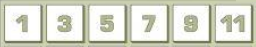
\includegraphics[width=0.3\textwidth]{progsample.png}

Tokiu atveju, jis galėtų pasakyti, jog \textit{aritmetinė progresija - tai skaičių seka, kuri didėja} ir nesuprasti, jog toks sąvokos supratimas nepilnas. Vadovėlyje pateikiamas apibrėžimas \textit{seka, kurios kiekvienas narys, pradedant antruoju, lygus prieš jį esančio ir to paties skaičiaus $d$ sumai} moksleivių dėmesio dažnai nesusilaukia. 

Ankstesniame skyrelyje pastebėjome, jog matematinės sąvokos turi išlaikyti griežtumą (jos turi būti \textbf{\textit{vienareikšmiškos}} ir \textbf{\textit{nedviprasmiškos}}). Tačiau lieka neaišku, kaip turėtų samprotauti moksleivis norėdamas užtikrinti, kad jo sąvokos supratimas taptų pilnu? Kaip mokytojui suformuluoti sąvokos apibrėžimą, kad jis ne tik išlaikytų matematinį griežtumą, bet būtų pateiktas taip suprantamai, kad susilauktų moksleivių dėmesio? 

Norėdami atsakyti į šiuos klausimus turime atsižvelgti ne tik į matematinio apibrėžimo griežtumo aspektą, bet ir \textbf{\textit{mokykliškumo}} aspektą. Apibrėžimo mokykliškumu laikome jo savybę būti suprantamu įvairių gebėjimų moksleiviams. Teorinė struktūra, kuri apima šiuos du aspektus, galėtų būti tokia:
\begin{itemize}
\item \fbox{Kategorijos įvardijimas} 
\item \fbox{Kategorijos požymio įvardijimas} 
\item \fbox{Apibrėžimo lankstumo įvertinimas: ar kategorija tikrai nurodyta teisingai?} 
\item \fbox{Apibrėžimo lankstumo įvertinimas: veiksmų, atliekamų su objektu, paaiškinimas pagal kategorijos požymį} 
\item \fbox{Apibrėžimo lankstumo įvertinimas: pavartotų sąvokų kiekis ir sudėtingumas}
\item \fbox{Apibrėžimo tinkamumo palyginimas: pasitikrinimas įvairiuose šaltiniuose}
\end{itemize}

Teorinės struktūros taikymo pavydys.

\fbox{Kategorijos įvardijimas} 

\texttt{Aritmetinė progresija - tai seka.}

\fbox{Kategorijos požymio įvardijimas} 

\texttt{Aritmetinė progresija - tai seka, {\color{red}{kuri didėja}}} - apibr. per \textbf{\textit{siauras}}, nes ji gali ir mažėti, pvz. \{1, 0, -1, -2, -3, -4\}

\texttt{Aritmetinė progresija - tai seka, {\color{red}{kuri didėja arba mažėja}}} - apibr. per\textbf{\textit{ platus}}, nes ne visos sekos tinka: seka $\{1, \frac{1}{2},\frac{1}{3}, \frac{1}{4}, \dots\}$ nėra laikoma aritmetine progresija.

\texttt{Aritmetinė progresija - tai seka, kuri didėja arba mažėja {\color{red}{vienodai}}} - apibr. per \textbf{\textit{platus}}, nes didėjimas arba mažėjimas gali būti dvejopas: kažkokiu skaičiumi arba kažkokiu kiekiu kartų. Pvz. $\{2, 4 ,6 ,8, 10,\dots\}$ būtų gerai, bet $\{2, 4 ,8 ,16,32,\dots\}$ būtų blogai.

\texttt{Aritmetinė progresija - tai seka, kuri didėja arba mažėja {\color{red}{kažkokiu skaičiumi}}} - apibr. tikslus, bet painus. Dažnas gali painioti, kuo skiriasi didėjimas kažkokiu skaičiumi arba kažkiek kartų, įsivaizduoti, kad tas skaičius arba kiekis gali būti tik netrupmeninis.

\texttt{Aritmetinė progresija - tai seka, kuri didėja arba mažėja {\color{red}{pastoviu skirtumu}}} - apibr. tikslus, bet painus, nes galima pasimesti, kieno tai skirtumas. Kalbama apie sekos didėjimą ir mažėjimą, o po to pereinama prie skirtumo, kuris gali būti tik sekos narių.

\texttt{Aritmetinė progresija - tai seka, kurios nariai didėja arba mažėja pastoviu skirtumu} - šį apibr. pretenduoja į tinkamą. Žinoma, norėtųsi patikslinti, kad kalbama būtent apie gretimų, o ne bet kurių narių skirtumą, tačiau pats didėjimas ir mažėjimas yra netiesioginė nuoroda į gretimų narių lyginimą (skirtumo radimą). Dėl panašių atvejų formuluojant apibrėžimus yra sunku pasiekti visišką lankstumą (ir tikslumą, ir aiškumą).

\fbox{Apibrėžimo lankstumo įvertinimas: ar kategorija tikrai nurodyta teisingai?} 

Tikriname: seka - tai sunumeruotų objektų rinkinys, kuriame objektai gali pasikartoti (\textit{angl. Vikipedija}). Vadinasi, aritmetinė progresija tikrai yra seka. 

\fbox{Apibrėžimo lankstumo įvertinimas: veiksmų, atliekamų su objektu, paaiškinimas pagal kategorijos požymį} 

Su aritmetine progresija įprasta atlikti šiuos veiksmus: rasti jos narių kiekį, $n$- tąjį narį, narių sumą, gretimų narių skirtumą. Šie veiksmai neprieštarauja apibrėžimui. Kategorijos požymis \textit{nariai didėja arba mažėja vienodu skirtumu} nurodo, kad visi įvardinti veiksmai gali būti atliekami tokiu eiliškumu:

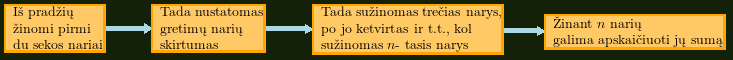
\includegraphics[width=\textwidth]{aritm_prog_eiga.png}

Vadinasi, apibrėžimas yra lankstus tuo požiūriu, kad jame atsispindi nuorodos į veiksmus, kuriuos galime atlikti su apibrėžiamu matematiniu objektu (aritmetine progresija).

\fbox{Apibrėžimo lankstumo įvertinimas: pavartotų sąvokų kiekis ir sudėtingumas}

Apibrėžime paminėtos sąvokos: \textit{seka, nariai, didėja, mažėja, pastovus, skirtumas}. Krinta į akis, kad prireikė pakankamai daug sąvokų.

\fbox{Apibrėžimo tinkamumo palyginimas: pasitikrinimas įvairiuose šaltiniuose}

\textit{Pastaba: angliška Vikipedija yra patikimesnė už lietuvišką.}
\begin{itemize}
\item Angliškoje Vikipedijoje rašoma, kad aritmetinė progresija - tai seka, kurios gretimų narių skirtumas yra pastovus. 

\item Lietuviškoje Vikipedijoje rašoma, kad aritmetinė progresija - tai tokia skaičių seka, kurios skirtumas tarp šalia esančių narių yra pastovus. 

\item Vadovėliuose \textit{Matematika Tau +, Matematika 11} ir \textit{ALGEBRA 9-10} beveik vienodai rašoma, kad aritmetinė progresija - tai seka, kurios kiekvienas narys, pradedant antruoju, lygus prieš jį esančio ir to paties skaičiaus $d$ sumai.
\end{itemize}

\textcolor{red}{
Atviri klausimai
\begin{itemize}
\item Patikimi matematinių sąvokų šaltiniai. Ar galime remtis vien matematikos vadovėliais? Ar galime remtis Vikipedija? O gal remtis kuo nors kitu?
\item Kuo remiantis vadovėlyje panaudotas ilgas apibrėžimas, kuriame atsispindi, kaip matematikos objektas sudaromas, yra geresnis už kitokį, trumpesnį apibrėžimą, kalbantį apie matematines objekto savybes? 
\item Kokios dar yra priežastys, dėl kurių matematiniai apibrėžimai moksleivių dėmesio nesusilaukia net mokant juos papildomai? 
\item Matematinių apibrėžimų griežtumo sąvoka. Ką vadiname griežtumu?
\end{itemize}}

\subsection{Trivialumo vaidmuo sąvokos sampratoje}
Atkreipkime dėmesį į subtilų skirtumą tarp dviejų apibrėžimų:
\begin{itemize}
\item \texttt{Aritmetinė progresija - tai seka, kurios nariai didėja arba mažėja pastoviu skirtumu.}
\item \texttt{Aritmetinė progresija - tai seka, kurios gretimų narių skirtumas yra pastovus.}
\end{itemize}

Reikia \textit{\textbf{aukštesnio pastabumo}} norint pajusti, kodėl šie apibrėžimai nevienodi. Pasirodo, jog teiginiai \textit{nariai didėja arba mažėja pastoviu skirtumu} ir \textit{gretimų narių skirtumas yra pastovus} reiškia ne tą patį. Dėmesį reikėjo atkreipti į tai, jog specialiu atveju, kai sekoje šis skirtumas yra lygus 0, ši seka pagal pirmąjį apibrėžimą nebūtų progresija, o pagal antrą būtų. Apibrėžimai prieštaringi. Kuris iš jų teisingas?
\begin{mdframed}[backgroundcolor=blue!10!white, linewidth=3pt]
\textit{\textbf{Trivialiais}} vadinami atvejai, kurie yra suvokiami kaip lengvi arba turintys labai paprastą struktūrą, tačiau negali būti ignoruojami apibrėžimuose, teoremose, taisyklėse ir kt.
\end{mdframed}

Minėtas specialus atvejis laikomas \textit{\textbf{trivialiu}}. Atsakymą į klausimą galima rasti \href{https://math.stackexchange.com/questions/1437413/can-a-arithmetic-progression-have-a-common-difference-of-zero-a-geometric-prog}{internete}:

\textit{Pagal susitarimą matematinėje kalboje apibrėžiant sąvoką pagal nutylėjimą yra priimtina įtraukti \textbf{trivialius} (*) atvejus, o tada, kai norime nurodyti, kad jie yra neįtraukti, pridedame nurodomuosius būdvardžius netrivialus arba, kaip šiuo atveju, (kalbant apie seką) nepastovus.}

{\small{(*) Išimtys pasitaiko, kai trivialūs atvejai reikalauja atskiro nagrinėjimo didesnėje dalyje teoremų, kuriose sąvoka vartojama. Pavyzdžiui Van der Waerden'o teoremoje ir jos apibendrinimuose.}}

Vadinasi tik antras apibrėžimas buvo teisingas. Pastebėkime, kad čia padėjo rėmimasis angliška Vikipedija.

\subsection{Matematikų indėlis į sąvokos sampratą}
Kitas \textit{\textbf{aukštesnio pastabumo}} reikalaujantis pavyzdys būtų aibės sąvoka. Vienas iš mokyklinėje matematikoje pasitaikančių pavyzdžių būtų realiųjų skaičių intervalas, su kuriuo moksleiviai supažindinami 8kl. Moksleiviams ir mokytojams pakaktų intervalą $(a; b)$ įsivaizduoti kaip visų skaičių, kurie yra tarp $a$ ir $b$, \colorbox{orange}{krūvą}, ir toks suvokimas būtų pakankamas mokyklinėje arba daugelyje aukštosios matematikos sričių. G. Kantoras (1845 - 1918), aibių teorijos atradėjas, aibę apibrėžė taip:

\textit{Aibė yra apibrėžtų, skirtingų mūsų pojūčiais ir mintimis suvokiamų objektų sukomplektavimas į visumą. Šie objektai vadinami tos aibės elementais} \textit{(angl. Wikipedia)}

Atkreipkime dėmesį, jog kategorija, apibrėžianti aibę, yra buitinė, o ne matematinė. Tai sako, jog aibės sąvoka yra arba primityvi, arba buitinė. Šiandien daugumoje šaltinių aibę laikyti \textit{\textbf{primityvia}} sąvoka pakanka tiek mokyklinėje, tiek aukštojoje matematikoje. Ją suvokiame ne griežtai, o intuityviai, todėl intuityviai suvokiame ir aibės savybes, tokias kaip galimybę turėti elementus arba lygumą su kita aibe, reiškiantį, jog kiekvienos iš lygintinų aibių elementai bus taip pat ir kitoje aibėje.

Nors aibės suvokimą kaip skirtingų elementų krūvą laikome pakankamai pilnu, tačiau matematikų tarpe jis pasirodė prieštaringas. Nustatyti, jog yra matematinių pavyzdžių, kai aibę laikyti elementų krūva yra prieštaringa, pareikalavo tokio \textit{\textbf{aukšto pastabumo}}, jog matematikai neatitikimų šiame apibrėžime nepastebėjo iki XXa. pr. Štai paradoksas, kurį 1903 metais aprašė Bertrand'as Russel'as:

\newtcolorbox{mybox}[1]{colback=blue!5!white,colframe=blue!75!black,fonttitle=\bfseries,title=#1}
\begin{mybox}{Russel'o paradoksas}
\begin{framed}
Aibę vadinsime:
\begin{itemize}
\item \textbf{\textit{nenormalia}}, jei ji yra savo paties narys
\item \textbf{\textit{normalia}}, jei ji nėra savo paties narys. 
\end{itemize}
\end{framed}

Štai pavyzdys, skirtas pailiustruoti, apie ką eina kalba:
\begin{enumerate}
\item Tarkim turim visų pasaulio arbatinukų aibę. Galite įsivaizduoti į milžinišką krūvą suneštus arbatinukus. Šioje krūvoje yra tik arbatinukai, vadinasi aibė nepriklauso sau pačiai. Taigi šiuo atveju pagal apibrėžimą turime, jog ką tik minėta arbatinukų aibė yra normali - ji nėra savo paties narys. 
\item Tarkim turim visų pasaulio nearbatinukų aibę. Taigi vėl galite įsivaizduoti visus pasaulio daiktus, kurie nėra arbatinukai, sumestus į krūvą. Šiuo atveju pati aibė (milžiniška krūva) taip pat yra nearbatinukas. Taigi ir visa ta milžiniška krūva priklauso nearbatinukų aibei. Pagal apibrėžimą turime, jog tokia nearbatinukų aibė yra nenormali, nes ji yra savo paties narys.
\end{enumerate}
Išnagrinėjęs šį pavyzdį skaitytojas turėtų įgyti intuiciją, kas yra normali ir nenormali aibės. Paradoksas jau netoli!
\newline
\newline
Dabar tarkim, jog turime aibę, kurią pažymėsime S, ir kurios nariai yra visos įmanomos normaliosios aibės (taigi S yra visų pasaulio normaliųjų aibių aibė). Nagrinėsime du atvejus:
\begin{enumerate}
\item Aibė S yra normali. Kadangi į aibę S patenka visos įmanomos normaliosios aibės, tai ji turi būti savo pačios narys. O pagal apibrėžimą, jei aibė yra savo paties narys - ji nenormali. Gavome, kad aibė S yra ir normali, ir nenormali, kas neįmanoma.
\item Aibė S  yra nenormali.  Kadangi į aibę S patenka visos įmanomos normaliosios aibės, o S nėra normali, tai S į save nepatenka. Bet jei nepatenka, tai nėra savo paties narys, o tuomet tokia aibė pagal apibrėžimą yra normali. Vis gi ir vėl gavome, kad aibė S yra ir normali, ir nenormali, kas neįmanoma.
\end{enumerate}
Štai ir paradoksas - aibė S nei normali, nei nenormali. 
\end{mybox}

Šis paradoksas sugriovė G. Kantoro be jokių ribojimų naudotą aibės sąvoką. Pagal Kantoro formuluotę egzistuoja matematiniai objektai, apie kuriuos negalime vienareikšmiškai pasakyti, ar jie aibės. Tai, ką nuveikė matematikai siekdami iš šios sąvokos pašalinti nevienareikšmiškumą, galėtų būti gera iliustracija, atspindinti kaip matematikos teiginių skirstymas į akivaizdžius ir neakivaizdžius yra susijęs su matematinių sąvokų apibrėžimu.

\begin{mdframed}[backgroundcolor=blue!10!white, linewidth=3pt]
\textit{\textbf{Aksiomomis}} laikomi teiginiai, kurie matematikų sutarimu yra pripažinti teisingais ir neraikalaujantys įrodymo. 
\textit{\textbf{Primityvių matematinių sąvokų}} ir teiginių, kuriuos susitarta laikyti akivaizdžiais, rinkinys yra laikomas \textit{\textbf{aksiomų sistema}}.\\
\end{mdframed}

Keletas matematikų pasiūlė naujas \textit{\textbf{aksiomų sistemas}}, kurios turėjo nusakyti, kokias savybes turi tenkinti aibė, kad tos savybės nebūtų prieštaringos, t.y. būtų išvengta paradoksų, panašių į aprašytąjį. Laiko išbandymus iki šiol sėkmingai atlaikė fiziko ir matematiko E. Zermelo (1871-1953) pasiūlytoji aibės sąvoką apibrėžianti \textit{\textbf{aksiomų sistema}}. Ją galima rasti šioje \href{http://www.math.tamu.edu/\~boas/courses/220-2003c/nov14.pdf}{nuorodoje.} Anot matematiko D. Hilberto, sėkmingas aibės sąvokos išgelbėjimas nuo prieštaringumo atidarė vartus matematikams į rojų, iš kurio jų niekas negali išvaryti. Šiandien aibė pagal susitarimą yra \textit{\textbf{primityvi sąvoka}}, o \textit{\textbf{aksiomų sistemos}} taikomos tik kontekstuose, kuriuose prireikia didesnio matematinio griežtumo.

\subsection{Aksiomų sistemų vaidmuo apibrėžimo formulavime}

Aksiomos yra prielaidos, kuriomis turi būti grindžiamas tolimesnis samprotavimas. Bet kurie teiginiai, išvesti iš aksiomų, įeinančių į aksiomų sistemą, turi būti neprieštaringi.  Pavyzdžiui Hilberto (1900m.) aksiomų sistemoje primityviomis sąvokomis laikomos sąvokos \textit{taškas}, \textit{tiesė}, \textit{plokštuma}, \textit{taško buvimas tarp dviejų taškų}, \textit{turėjimas (savyje)} arba \textit{buvimas ant} ir \textit{panašumas}. \href{http://folk.uio.no/bjoernj/kurs/4510/hilberteng.pdf}{Šioje aksiomų sistemoje} iš viso yra 20 aksiomų. Štai keletas jų:
\begin{itemize}
\item Tarp trijų taškų, kurie yra ant vienos tiesės, egzistuoja ne daugiau nei vienas taškas, esantis tarp kitų dviejų.
\item Bet kuriems dviems taškams egzistuoja tiesė, turinti tuos taškus.
\item Jei taškas $A$ yra ne ant tiesės $a$, tai plokštumoje egzistuoja ne daugiau nei viena tiesė, nekertanti tiesės $a$ ir turinti tašką $A$
\end{itemize} 

Grįžkime prie mūsų turėto problematiško atkarpos sąvokos apibrėžimo.

\colorbox{green}{Atkarpa} - tai \colorbox{cyan}{tiesės} \fbox{dalis}, \colorbox{yellow}{apribota} \fbox{dviejų} \colorbox{cyan}{taškų} ir \colorbox{cyan}{esanti tarp} jų.

Pagal Hilberto aksiomų sistemą šis apibrėžimas būtų prieštaringas, nes šioje aksiomų sistemoje nėra apibrėžta, ką reiškia sąvoka \textit{apribojimas}. Be to \textit{taško buvimas tarp dviejų taškų} yra primityvi sąvoka, o \textit{tiesės dalies buvimas tarp dviejų taškų} yra sąvoka, kuriai reiktų atskiro apibrėžimo. Naudodamiesi Hilberto pasiūlytomis primityviomis sąvokomis nurodymą \textit{tiesės dalis yra tarp dviejų taškų} pakeiskime nurodymu, kad \textit{tiesės dalis yra sudaryta iš visų taškų, esančių tarp dviejų duotųjų}:

\begin{itemize}
\item Atkarpa - tai tiesės dalis, apribota dviejų taškų ir sudaryta iš visų taškų, esančių tarp jų.
\end{itemize}

Dabar prieštaringas žodis ,,apribota'' jau nebėra būtinas:

\begin{itemize}
\item Atkarpa $AB$ - tai tiesės dalis, sudaryta iš visų taškų, esančių tarp taškų $A$ ir $B$.
\end{itemize}

\subsection{Sąvokų abstraktumo savybės vaidmuo sąvokos sampratoje}
Hilberto aksiomų sistemoje atkarpą siūloma apibrėžti taip:

\texttt{\textbf{Atkarpa $AB$ - tai aibė taškų, turinti taškus $A$, $B$ ir taškus, kurie yra tarp jų.}}

Tačiau šio apibrėžimo negalime laikyti \textit{\textbf{mokykliniu}}, nes aibės sąvoka yra per daug abstrakti moksleiviams penktoje klasėje. Tai galbūt parodo, kodėl mokykliniame vadovėlyje atkarpą apibūdina kaip tiesės dalį, o ne kaip taškų aibę.

Kitos žemesnių klasių moksleiviams per sudėtingos sąvokos galėtų būti \textbf{\textit{skaičius, kintamasis}} ir \textbf{\textit{objektas}}. Tinkamas šių sąvokų nesupratimas dažnai domino principu blokuoja tolimesnių sąvokų supratimą bent jau tiek, kiek jo reikia mokyklinei programai. Tai iliustruoja skyriaus pradžioje pateiktas pavyzdys, kad klaidinga skaičiaus sąvokos samprata trukdo suprasti šaknies sąvoką. 

\texttt{\textbf{Kintamasis - tai skaičių aibės (vadinamos jo kitimo sritimi), elementas}}.

\href{http://norvaisa.lt/matematika/mokykline-matematika/kas-yra-skaicius/}{Apie skaičiaus sampratą mokykloje}

\href{http://norvaisa.lt/matematika/kas-yra-matematika/iracionaliuju-skaiciu-priesistorija-2/}{Apie skaičiaus sampratos istorinį kitimą detaliai}

\textcolor{red}{
Atviri klausimai
\begin{itemize}
\item Nagrinėkime uždavinį \textit{Aš sugalvojau skaičių, tada jį padauginau iš 2 ir pridėjau 1, o po to tai atlikau dar trissyk. Gavau 47. Koks buvo skaičius?} Stropus, gana aukštus įvertinimus iš matematikos gaunantis šeštokas tvirtina manantis, jog $2x+1$ yra tas pats 3, kur $x$ žymi ieškomą skaičių uždavinyje. Kaip nenaudodami kintamojo apibrėžimo paaiškintumėte, kaip suprasti užrašo $2x+1$ prasmę? Kas galėjo nulemti šį klaidingą moksleivio manymą?
\item Kiek sąvokose išlaikyti matematiškumo, ir kiek mokykliškumo? Klausimas atviras.
\item Kiek mokykloje skirti dėmesio sąvokų nagrinėjimui? Mano atsakymas: tiek, kiek supratimas nebūtų trukdantis suprasti kitas mokyklines sąvokas.
\item Kokie būtų pavyzdžiai be Piaget teorijos, pagrindžiantys sąvokų \textit{skaičius, aibė, kintamasis, objektas} per didelį sudėtingumą žemesniųjų klasių moksleiviams?
\end{itemize}}

\subsection{Pastebėtos kliūtys, trukdančios formuotis sąvokos sampratai}
\begin{itemize}
\item Gebėjimas interpretuoti matematinių sąvokų junginius. Pavyzdžiai:
\begin{itemize}
\item Mokinys supranta skaitmens ir sumos sąvokas, tačiau negali rasti duoto skaičiaus skaitmenų sumos.
\item Mokinys negali sudaryti skaitinių reiškinių, atitinkančių skaičių 3 ir 6 kvadratų sumą, sumos kvadratą, sumos ir skirtumo sandaugą ir pan.
\item Užduotys, sudarytos iš 3 matematinių sąvokų su papildomais požymiais dar sunkesnės. Pavyzdžiui duotos nelygybės natūraliųjų sprendinių radimas duotame intervale.
\end{itemize}
\item Gebėjimas interpretuoti sąryšius tarp matematinių objektų. Pavyzdžiui teiginys \textit{statinis prieš $30^o$ laipsnių kampą lygus pusei įžambinės} yra nesuprantamas be pagalbos.
\item Apibrėžiamų objektų atskyrimo trūkumas (recognition).  Gyvosios patirties nebuvimas trukdo ne tik tikslinti regimo objekto kategoriją, bet ir ją įvardyti. 
\item Gebėjimas skirti, su kokių kategorijų objektais gali būti atliekami aritmetiniai veiksmai. 
\end{itemize}
\section{Enkapsuliacija}
\subsection{Gebėjimas atlikti žingsnius, reikalingus procedūroms atlikti}
Apie enkapsuliaciją daug nekalbėsime, tik pabandysime panagrinėsime pora procedūrų ir sunkumus, su kuriais susiduria moksleiviai norėdami jas išmokti atlikti.
\begin{enumerate}
\item Reikia apskaičiuoti $\frac{24}{48}$. 

Pirmasis moksleivis šios pocedūros atlikti negeba. Jis perrašo trupmeną kaip $\frac{2 \cdot 2 \cdot 2 \cdot 3}{2 \cdot 2 \cdot 2 \cdot 2 \cdot 3}$. Tačiau suprastinęs vienodus daugiklius jis pastebi, jog tuomet skaitiklyje nelieka jokių daugiklių. Susidariusi situacija nesuprantama. Vėliau moksleiviui paaiškinus, jog skaitiklyje dvejetą pakeitę sandauga $2 \cdot 1$, jis procedūrą atlikti geba ir atsimena, kaip ją atlikti po savaitės. 

Antrasis moksleivis procedūrą atlikti geba. Jis sumažina ir skaitiklį ir vardiklį po 2, tada po 2, tada po 2, tada po 3 kartus ir gauna $\frac{1}{2}$
\item Reikia apskaičiuoti $\sqrt{50}$. Moksleivis procedūros atlikti negeba. Tad iš pradžių skaičiuojame $\sqrt{100}$. Procedūros aiškinimo eiga: 
\begin{itemize}
\item Pošaknio skaidymas turi sunkių vietų. Moksleivis nesupranta, jog tai, jog 100 padaliję iš 2, tada 2, tada 5, gausime 5, reiškia, kad $100=2\cdot 2\cdot 5\cdot 5$. 
\item Dabar moksleivis skaičiuodamas $\sqrt{100}$ gauna 10. Gautasis rezultatas niekaip nesisieja su skaidymu daugikliais.
\item Moksleiviui paaiškinama šaknies apibrėžimas ir yra pasiūloma įsitikinti, jog skaičių $2\cdot 5$ sudauginę su savimi gausime $2\cdot 2\cdot 5\cdot 5$. Moksleiviui nesuprantama, kodėl pasiūlytas teiginys galioja. Pasiūlius sandaugoje sukeisti du vidurinius daugiklius moksleiviui teiginys tampa suprantamu.
\item Moksleiviui pasiūloma įsitikinti, jog traukiant šaknį daugiklių grupė sumažėja perpus ir moksleiviui šis teiginys suprantamas.
\end{itemize}
Dabar pereiname prie skaičiaus $\sqrt{50}$. Dabar moksleivis išskaido skaičių 50 pirminiais dauginamaisiais ir gautą daugiklių grupę dalija į dvi lygias dalis, tačiau nežino, ką atlikti su daugikliu 2, kuris yra tik vienas. Moksleiviui pasiūloma sugalvoti tokį daugiklį $x$, kad $x\cdot x=2$. Pirmoji jam kilusi mintis yra 1, tačiau jis greit įsitikina, jog tai netiesa. Skaičius 1,5 taip pat netinka. Galiausiai moksleiviui prireikia vėl priminti šaknies apibrėžimą, kad galėtume skaičių 2 išreikšti sandauga $\sqrt{2}\cdot \sqrt{2}$.

Panašiai su įvairiais sufleriais moksleivis sprendžia likusius panašius pavyzdžius. Po savaitės jis procedūros atlikti negeba.
\end{enumerate}
\section{Kuo remiantis yra įvedamos matematikos sąvokos vadovėliuose?}
\subsection{Kinietiškas pavyzdys}
\textit{Pateiksime ištrauką iš bestseleriu tapusios knygos}
Pagrindinę mokytojo vadovo dalį sudaro diskusija apie vadovėlio temas ir potemes, einanti skyrius po skyriaus. Diskusija apie kiekvieną temą yra fokusuota ties šiais klausimais:
\begin{itemize}
\item Su kokia sąvoka yra susieta pristatoma tema?
\item Kokios yra sunkiausios vietos mokant sąvoką?
\item Kokios yra svarbiausios vietos mokant sąvoką?
\item Kur dažniausiai suklysta ir susipainioja mokiniai besimokant sąvoką?
\end{itemize}
\subsection{Lietuviškas pavyzdys}
\textit{Pateiksime ištrauką iš Viktorijos Sičiūnienės pirmos knygos ,,Matematikos didaktika''}
Mokyklinėje matematikoje sąvokos yra apibrėžiamos įvairiai: klasikiniu apibrėžimu, genetiniu apibrėžimu arba pateikiant sąvokos aprašymą.
\begin{itemize}
\item Apibūdinant sąvoką klasikiniu apibrėžimu yra nurodoma sąvokos giminė (rūšis) ir
rūšinis požymis. Sąvokos klasikinio apibrėžimo pavyzdžiai: ,,Lygiagretainiu (apibrėžiama sąvoka) vadiname keturkampį (daugiakampio rūšis), kurio priešingos kraštinės lygiagrečios (rūšinis požymis)''; ,,Tiesė (figūros rūšis), kurios atžvilgiu figūra yra simetriška
pati sau (rūšinis požymis), vadinama tos figūros simetrijos ašimi'' (apibrėžiama sąvoka).
\item Kai yra apibūdinama, kaip sudaromas (gautas) apibrėžiamas objektas, tai sakoma,
kad sąvoka apibrėžiama genetiškai. Sąvokos genetinio apibrėžimo pavyzdžiai: ,,Kūnas,
gautas stačiakampį sukant apie ašį, kurioje yra jo kraštinė, vadinama ritiniu“; ,,Du algebriniai reiškiniai, susieti lygumo ženklu, sudaro lygybę.''
\item Kartais vienu sakiniu pateikiamas sąvokos apibrėžimas esti labai painus, sunkiai
mokiniams suprantamas. Tada jį galima (o kartais ir tikslinga) pakeisti sąvokos aprašymu, kuris tuo pačiu suteikia ir papildomos informacijos apie apibrėžiamą sąvoką.
Pavyzdžiui, lygčių sistemos sprendimo sudėties būdu algoritmą galima aprašyti taip:
,,Pastebėjus, kad abiejų lygčių koeficientai prie kurio nors nežinomojo yra vienas kitam
priešingi skaičiai, lygčių sistemą galima spręsti sudėties būdu. Jo esmė – vieno nežinomojo pašalinimas sudedant lygtis.''  Kaip reikia dauginti trupmeninius reiškinius, sužinome iš tokio aprašymo: ,,Trupmeniniai reiškiniai dauginami kaip paprastosios trupmenos. Skaitiklyje rašoma skaitiklių sandauga, o vardiklyje – vardiklių sandauga.''
\end{itemize}
\section{Kai kurių sąvokų rinkinys}
\subsection*{Bendros sąvokos}
Pasiūlysime apibrėžimus sąvokų, kurios yra dažnos kitų sąvokų apibrėžimuose

$\fbox{Matematika}$ - tai kultūros dalis, samprotavimu įprasminanti žmonijos praktinę ir pažintinę veiklą.\par
\fbox{Objektas} (bendrinėje kalboje) - tai, į ką nukreipta mūsų pažintinė veikla.\par
\fbox{Matavimas} - lygintino skaičiaus priskyrimas objekto ar reiškinio savybei.\par
\fbox{Skaičiavimas} - skaičiaus priskyrimas baigtinės aibės objektų kiekiui.\par
\fbox{Kvantifikavimas} - skaičiaus priskyrimas savybei, suvokiamai per juslę, vaizduotę ar kitaip. Matavimas yra vienas iš kvantifikavimo pavyzdžių.\par
\fbox{Kvantorius} - kvantifikavimą išreiškiantis žodis pvz. \textit{kiekvienas, kai kurie, daug, keletas, pusė, du, egzistuoja, visiems} ir t.t. \par
\fbox{Skaičius} - matematinis objektas, kurio paskirtis yra skaičiuoti, matuoti arba žymėti.\par
\fbox{Kiekis} - skaičiavimo rezultatas.\par
\fbox{Dydis} - 1) skaičiavimo arba matavimo rezultatas (atsako į klausimą \textit{kiek?}) 2) lygintina savybė. \textit{Pastaba: ją dažniausiai apibūdina neskaičiuotini daiktavardžiai}\par
\fbox{Matmuo} - savybė, kuri yra matuojama. (atsako į klausimą \textit{kas matuojama?})\par
\fbox{Matavimo vienetas} - tai bendru sutarimu apibrėžtas dydis, naudojamas kaip etalonas tam tikram matmeniui skaičiuoti. (kuo matuojame?)\par
\fbox{Narys} - tai matematinis objektas, dažniausiai tam tikro reiškinio ar veiksmo komponentas \par
\fbox{Formulė} - tai tam tikras prasmę turinčių matematinių simbolių rinkinys \par
\fbox{Veiksmas} arba \fbox{Operacija} - procedūra, kuomet panaudojant vieną ar kelis narius yra gaunamas kitas narys.\textit{ Pavyzdžiai: šaknies traukimas iš skaičiaus, dviejų skaičių atimtis, trupmenos apvertimas, kvadratinės lygties sprendinių gavimas, funkcijos išvestinės skaičiavimas, vektoriaus normavimas, matricos transponavimas.}\par
\fbox{Veiksmo rezultatas} - tai narys, gautas atlikus tam tikrą operaciją. \par
\fbox{Atsakymas} - tai kokios nors problemos ar uždavinio sprendimo rezultatas.\par
\fbox{Kintamasis} - tai žymuo, kuriuo žymimas bet kuris elementas iš kokios nors aibės. \textit{Pavyzdžiui apskritimo spindulį žymime raide $r$, kur $r$ yra bet kuris skaičius iš teigiamų realiųjų skaičių aibės.} \par
\fbox{Apribotas kintamasis} - tai kintamasis, kuriame nėra prasmės įstatyti konkretų objektą iš jo kitimo srities. Pvz. kintamasis $x$ šičia bus apribotas $\{x\in \mathbb{R}: x>3\}$, $\displaystyle \lim_{x\to 3}\sqrt{x}=3$, $\displaystyle \int_{0}^{1}x^3dx$ \par
\fbox{Laisvasis kintamasis} - tai kintamasis, kuriame įstačius konkretų objektą iš jo kitimo srities atsiranda nauja prasmė. Pvz. kintamasis $y$ šičia bus laisvasis $y\in\{x\in \mathbb{R}: x>3\}$, $\displaystyle \lim_{x\to 3}\sqrt{x}=y$, $\displaystyle \int_{0}^{y}x^3dx$ \par
\fbox{Reikšmių sritis} - tai aibė, kuriai priklauso tam tikras kintamasis\par
\fbox{Reiškinys} - tai matematinė frazė, sudaryta iš skaičių, kintamųjų, aritmetinių operacijų ir kitų matematinių objektų. Konkretus skaičius taip pat yra reiškinys. Pavyzdžiui $x+8$ atitinka frazę ,,skaičius plius aštuoni''. \par
\fbox{Nežinomasis} - tai kintamasis, kurio reikšmės ieškojimas yra prasmingas.\par
\fbox{Lygybė} - 1) tai matematinis sakinys, kuria nurodoma, kad dvi skirtingos išraiškos yra to paties skaičiaus vardai. Pavyzdžiui $2+5 = 3+4$ 2) tai naujo matematinio žymėjimo apibrėžtis. Pavyzdžiui $a^n=\underbrace{a\cdot a\cdot\dots\cdot a}_n$\par
\fbox{Lygtis} - tai lygybė, kuriai yra prasminga ieškoti nežinomojo reikšmes, su kuriomis ji tampa teisinga.\par
\fbox{Skliaustai} - tai matematinis žymėjimas, įvardijantis tam tikros operacijos pirmumą.

\subsection*{Kai kurios statistinės sąvokos}

\fbox{Populiacija} - tai panašių įvykių ar elementų grupė, numatyta tam tikram tyrimui. \par
\fbox{Imtis} - tai duomenų aibė, atrinkta iš populiacijos pagal tam tikrą procedūrą. \par
\fbox{Imties reikšmės} - tai imties narių matavimo rezultatai \par
\fbox{Statistika} - 1) mokslas ape duomenis; 2) duomenų imties charakteristika \par
\fbox{Vidurkis} - duomenų imties charakteristika, parodanti apie kurį skaičių svyruoja imties reikšmės. \par
\fbox{Dispersija} - duomenų imties charakteristika, parodanti, kaip toli nuo vidurkio išsidėsčiusios (išsibarsčiusios) jo įgyjamos reikšmės\par
\fbox{Grafikas} - ? \par
\fbox{Diagrama} - ?

\subsection*{Sąvokos apie funkciją}

\fbox{Funkcija} - tai atitiktis, pagal kurią (nebūtinai kiekvienam) skaičiui x iš realųjų skaičių aibės egzistuoja kitas jį atitinkantis realusis skaicius, žymimas f(x). \textit{Pastaba: tai nepilnas apibrėžimas, nes manoma, kad jį tikslų suvokti įmanoma tik tolesniame funkcijų nagrinėjime}\par
\fbox{Funkcija} - tai , pagal kurią kiekvienam skaičiui $x$, priklausančiam jos apibrėžimo sričiai (vadinamam jos argumentu), egzistuoja kitas jį atitinkantis realusis skaičius, žymimas $f(x)$ (vadinamas jos reikšme taške $x$). \textit{Pastaba: tai pilnas funkcijos apibrėžimas}\par
\fbox{Funkcijos grafikas} - tai aibė visų koordinačių plokštumos taškų, kurių abscisės lygios argumento $x$ reikšmėms, o ordinatės - atitinkamoms funkcijos reikšmėms. \par
\fbox{Funkcijos apibrėžimo sritis} - tai aibė funkcijos argumento reikšmių, su kuriomis funkcija įgyja kokią nors reikšmę. \par
\fbox{Funkcijos grafiko eskizas} - tai apytikslė funkcijos grafiko forma, iš kurios nebūtinai atsiskleidžia funkcijos reikšmės josargumentams (jai gauti naudojamas ne vien taškų žymėjimas koordinačių plokštumoje, bet ir kiti metodai) \par
\fbox{Funkcijos grafiko transformacija} - tai taisyklė, pagal kurią tam tikras funkcijos argumentų arba jos įgyjamų reikšmių pakeitimas atitinka (jam būdingą) funkcijos grafiko pokytį.
\end{document}